\documentclass{beamer}
% \mode<presentation>
\setbeamertemplate{navigation symbols}{}
\let\tempone\itemize
\let\temptwo\enditemize
\renewenvironment{itemize}{\tempone\addtolength{\itemsep}{0.5\baselineskip}}{\temptwo}
\usepackage{beamerthemeshadow}
\usepackage{tikz}
\usepackage{bbm}
\usepackage{hyperref}
\usepackage{natbib}
\usepackage{pgffor}
\usepackage{booktabs}
\usepackage{graphicx}
\usepackage{amssymb}
\usepackage{tabularx}
\usepackage{tikz,etoolbox}
\usepackage{tikz,amsmath,siunitx}
\usetikzlibrary{arrows,snakes,backgrounds,patterns,matrix,shapes,fit,calc,shadows,plotmarks}
\newcommand{\softmax}{\mathrm{softmax}}
\usepackage[normalem]{ulem}
\newcommand\tst{% thick strike through  %% from http://tex.stackexchange.com/questions/134088/mis-alignment-of-columns-in-tabular-environment-when-using-ulem-and-beamer
  \bgroup%
  \markoverwith{\textcolor{red}{\rule[1.1ex]{1pt}{0.8pt}}}%
  \ULon%
}

\AtBeginSection[]
{
  \begin{frame}
  \frametitle{Contents}
  \tableofcontents[currentsection]
  \end{frame}
}

\usepackage{subcaption}
% \usepackage{url}
% \usepackage{hyperref}
\usepackage[absolute,overlay]{textpos}
\usepackage{pgf}
\usepackage{latexsym}
\usepackage{amsfonts}
\usepackage{amssymb}
\usepackage{amsthm}
\usepackage{algorithm}
\usepackage{amsmath}
\usepackage{tabularx}
\usepackage{xcolor}
\usepackage[absolute,overlay]{textpos}
\usetikzlibrary{shapes,arrows,positioning,automata,positioning,spy,matrix,scopes,chains}
\newcommand{\digs}[2]{\hphantom{999}\llap{#1}\,+\,\hphantom{999}\llap{#2}}
\setbeamersize{text margin left=6mm}
\setbeamersize{text margin right=6mm}
\renewcommand{\insertnavigation}[1]{}
\setbeamertemplate{headline}{}
\setbeamertemplate{footline}{}
\usefonttheme{professionalfonts}
\setbeamercovered{transparent}
\mode<presentation>
\linespread{1.25}
\DeclareMathOperator{\Tr}{Tr} 

\usepackage{color}
\usepackage{multirow}
\usepackage{rotating}
\usepackage[all,dvips]{xy}
\usepackage{colortbl}
\usepackage{graphicx}
\usepackage{verbatim}
\usepackage{framed}
\usepackage{natbib}
\usepackage[labelformat=empty]{caption}
\newcommand{\air}{\vspace{0.25cm}}
\newcommand{\mair}{\vspace{-0.25cm}}

\setbeamertemplate{navigation symbols}{}%remove navigation symbols
\renewcommand{\rmdefault}{crm}
\newcommand{\lnbrack}{{\normalfont [}}
\newcommand{\rnbrack}{{\normalfont ]}\thinspace}
\newcommand{\lbbrack}{\textcolor{red}{\textbf{[}}}
\newcommand{\rbbrack}{\textcolor{red}{\textbf{]}}\thinspace}
\definecolor{vermillion}{RGB}{213,94,0}
\newcommand{\given}{\,|\,}
\definecolor{orange}{RGB}{230,159,0}
\definecolor{skyblue}{RGB}{86,180,233}
\definecolor{bluegreen}{RGB}{90,143,41}
% \definecolor{bluegreen}{RGB}{0,158,115}
\definecolor{myyellow}{RGB}{240,228,66} % i dunno if this is the same as standard yellow
\definecolor{myblue}{RGB}{0,114,178}
\definecolor{vermillion}{RGB}{213,94,0}
\definecolor{redpurple}{RGB}{204,121,167}
\definecolor{lightgrey}{RGB}{234,234,234}

\newcommand{\clust}{\ensuremath{\mathrm{clust}}}
\newcommand{\loc}{\ensuremath{\mathrm{loc}}}
\newcommand{\nicein}{\ensuremath{\,{\in}\,}}
\newcommand{\niceq}{\ensuremath{\,{=}\,}}
\newcommand{\uc}{\ensuremath{\mathrm{c}}}
\newcommand{\hc}{\boldh_{\uc}}
\newcommand{\cb}{\boldb_{\mathrm{\uc}}}
\newcommand{\cW}{\boldW_{\mathrm{\uc}}}

\newcommand{\ha}{\boldh_{\ua}}
\newcommand{\hp}{\boldh_{\up}}
% \newcommand{\hc}{\boldh_{\mathrm{c}}}


\def\kargmax{\operatornamewithlimits{K-arg\,max}}
%\DeclareMathOperator{\topK}{topK}
\def\topK{\operatornamewithlimits{topK}}
\DeclareMathOperator{\suk}{succ}
\newcommand{\longpfx}[1]{\ensuremath{w_1 \cdots w_{#1}}}
\newcommand{\longgoldpfx}[1]{\ensuremath{y_1 \cdots y_{#1}}}
\newcommand{\pfx}[1]{\ensuremath{w_{1:{#1}}}}
\newcommand{\goldpfx}[1]{\ensuremath{y_{1:{#1}}}}
\newcommand{\beampred}[2]{\ensuremath{\hat{y}_{1:{#1}}^{({#2})}}}
\newcommand{\boldx}{\mathbf{x}}

\usetikzlibrary{positioning}
% \setbeamerfont{alerted text}{series=\bfseries}
% \setbeamerfont{structure}{series=\bfseries}
% Needed for diakgrams.
\def\im#1#2{
  \node(#1) [scale=#2]{\pgfbox[center,top]{\pgfuseimage{#1}}
};}
% \input{pictures_header}


  \usetheme{Frankfurt}
  \useinnertheme{rectangles}

  \setbeamersize{text margin left = 1.5em}

  \setbeamercolor{background canvas}{fg=black,bg=white}
  \setbeamercolor{structure}{bg=orange!60!white}
  \setbeamercolor{block title}{bg=structure.bg,fg=structure.fg}
  \setbeamercolor{block body}{bg=structure.bg!40!background canvas.bg}

  \setbeamertemplate{navigation symbols}{}

  \setbeamertemplate{blocks}[default]
  \setbeamerfont{item}{size=\large,series=\bfseries}
  \setbeamertemplate{title page}[default][rounded=false,shadow=false]   
  \setbeamercovered{transparent=8}

\title[]{The State of Neural Summarization}


\author[Alexander Rush]{Alexander Rush } 

\institute[Harvard SEAS]{ \\
  \begin{center}
    \includegraphics[width=1.3cm]{seas}
  \end{center}

  \begin{center}
    \includegraphics[height=1.5cm]{samsung}
  \end{center}
  
}
\date{}
% \usetheme{Madrid}

\newcommand{\enc}{\mathrm{src}}
\newcommand{\xvec}{\mathbf{x}}
\newcommand{\yvec}{\mathbf{y}}
\newcommand{\wvec}{\mathbf{w}}
\newcommand{\cvec}{\mathbf{c}}
\newcommand{\zvec}{\mathbf{z}}
% \newcommand{\mcY}{\mathcal{Y}}
% \newcommand{\mcV}{\mathcal{V}}
\newcommand{\context}{\mathbf{w}_{\mathrm{c}}}
\newcommand{\embcontext}{\mathbf{\tilde{w}}_{\mathrm{c}}}
\newcommand{\inpcontext}{\mathbf{\tilde{x}}}
\newcommand{\start}{\mathbf{\tilde{y}}_{\mathrm{c0}}}
\newcommand{\End}{\mathrm{\texttt{</s>}}}

\newcommand{\Uvec}{\mathbf{U}}
\newcommand{\Evec}{\mathbf{E}}
\newcommand{\Gvec}{\mathbf{G}}
\newcommand{\Fvec}{\mathbf{F}}
\newcommand{\Pvec}{\mathbf{P}}
\newcommand{\pvec}{\mathbf{p}}
\newcommand{\Qvec}{\mathbf{Q}}
\newcommand{\Vvec}{\mathbf{V}}
\newcommand{\Wvec}{\mathbf{W}}
\newcommand{\hvec}{\mathbf{h}}
% \newcommand{\reals}{\mathbb{R}}

\newcommand{\Cite}[1]{{\footnotesize \citep{#1}}}
\newcommand{\TT}[1]{{\footnotesize\tt{#1}}}
\newcommand{\boldw}{\boldsymbol{w}}
\newcommand{\boldu}{\boldsymbol{u}}
\newcommand{\boldv}{\boldsymbol{v}}
\newcommand{\boldb}{\boldsymbol{b}}
\newcommand{\boldW}{\boldsymbol{W}}
\newcommand{\boldh}{\boldsymbol{h}}
\newcommand{\boldg}{\boldsymbol{g}}
\newcommand{\ua}{\ensuremath{\mathrm{a}}}
\newcommand{\up}{\ensuremath{\mathrm{p}}}
%\newcommand{\bphi}{\ensuremath{\mathbf{\phi}}}
\newcommand{\bphi}{\boldsymbol{\phi}}
\newcommand{\btheta}{\boldsymbol{\theta}}
\newcommand{\mcY}{\mathcal{Y}}
\newcommand{\mcX}{\mathcal{X}}
\newcommand{\mcC}{\mathcal{C}}
\newcommand{\mcA}{\mathcal{A}}
\newcommand{\mcV}{\mathcal{V}}
\newcommand{\trans}{\ensuremath{\mathsf{T}}}
\def\argmin{\operatornamewithlimits{arg\,min}}
\def\argmax{\operatornamewithlimits{arg\,max}}
\newcommand{\reals}{\ensuremath{\mathbb{R}}}

\newcommand{\aphi}{\boldsymbol{\phi}_{\mathrm{a}}}
\newcommand{\pwphi}{\boldsymbol{\phi}_{\mathrm{p}}}
\newcommand{\squigaphi}{\widetilde{\boldsymbol{\phi}}_{\mathrm{a}}}
\newcommand{\squigpwphi}{\widetilde{\boldsymbol{\phi}}_{\mathrm{p}}}

\newcommand{\aW}{\boldW_{\mathrm{\ua}}}
\newcommand{\pW}{\boldW_{\mathrm{\up}}}

\newcommand{\ab}{\boldb_{\mathrm{\ua}}}
\newcommand{\pb}{\boldb_{\mathrm{\up}}}

\newcommand{\Da}{d_{\mathrm{a}}}
\newcommand{\Dp}{d_{\mathrm{p}}}

% \newcommand{\ha}{\boldh_{\ua}}
% \newcommand{\hp}{\boldh_{\up}}

\newcommand{\ourmodel}{This work}
\newcommand{\zro}{{\color{white}0}}

\newenvironment{thm}[1]
{\begin{block}{Theorem #1}}
{\end{block}}
\makeatletter % to change template
    \setbeamertemplate{headline}[default] % not mandatory, but I though it was better to set it blank
    \def\beamer@entrycode{\vspace*{-\headheight}} % here is the part we are interested in :)
\makeatother

\def\argmax{\operatornamewithlimits{arg\,max}}
\def\kargmax{\operatornamewithlimits{K-arg\,max}}

\begin{document}

\begin{frame}
  \titlepage
\end{frame}


\begin{frame}{Sequence-to-Sequence}

  \begin{itemize}
  \item \alert<2>{Machine Translation} \Cite{kalchbrenner2013recurrent,sutskever2014sequence, Cho2014, bahdanau2014neural,luong15effective} 
    \air

   
  \item Question Answering \Cite{Hermann2015} 
  \item Conversation \Cite{Vinyals2015} \Cite{Serban2016}
  \item Parsing \Cite{vinyals15grammar}
  \item Speech \Cite{Chorowski2015,Chan2015}
  \item Caption Generation \Cite{karpathy2015deep,Xu2015,Vinyals2015b}
  \item Video-Generation \Cite{Srivastava2015a}
  \item NER/POS-Tagging \Cite{Gillick2016}
  \item Summarization \Cite{Rush2015} 
    \air 

  \end{itemize}  
\end{frame}

\section{Sequence-to-Sequence}

\begin{frame}
  \begin{center}
    \alert{Seq2Seq Neural Network Toolbox}
    \air 
  \end{center}
  \begin{center}
    \begin{tabular}{cclll}
      \structure{Embeddings} & & sparse features &$\Rightarrow$& dense features \\\\
      \structure{RNNs} & & feature sequences & $\Rightarrow$ &dense features \\\\
      \structure{Softmax} & & dense features & $\Rightarrow$ & discrete predictions \\
    \end{tabular}
  \end{center}
\end{frame}

\begin{frame}
  \begin{center}
    \begin{tabular}{cclll}
      \structure{Embeddings} & & sparse features & $\Rightarrow$ & dense features \\\\
    \end{tabular}
  \end{center}

  \begin{center}
    \includegraphics[width=7cm]{emb}
  \end{center}
\end{frame}

\begin{frame}
  \begin{center}
    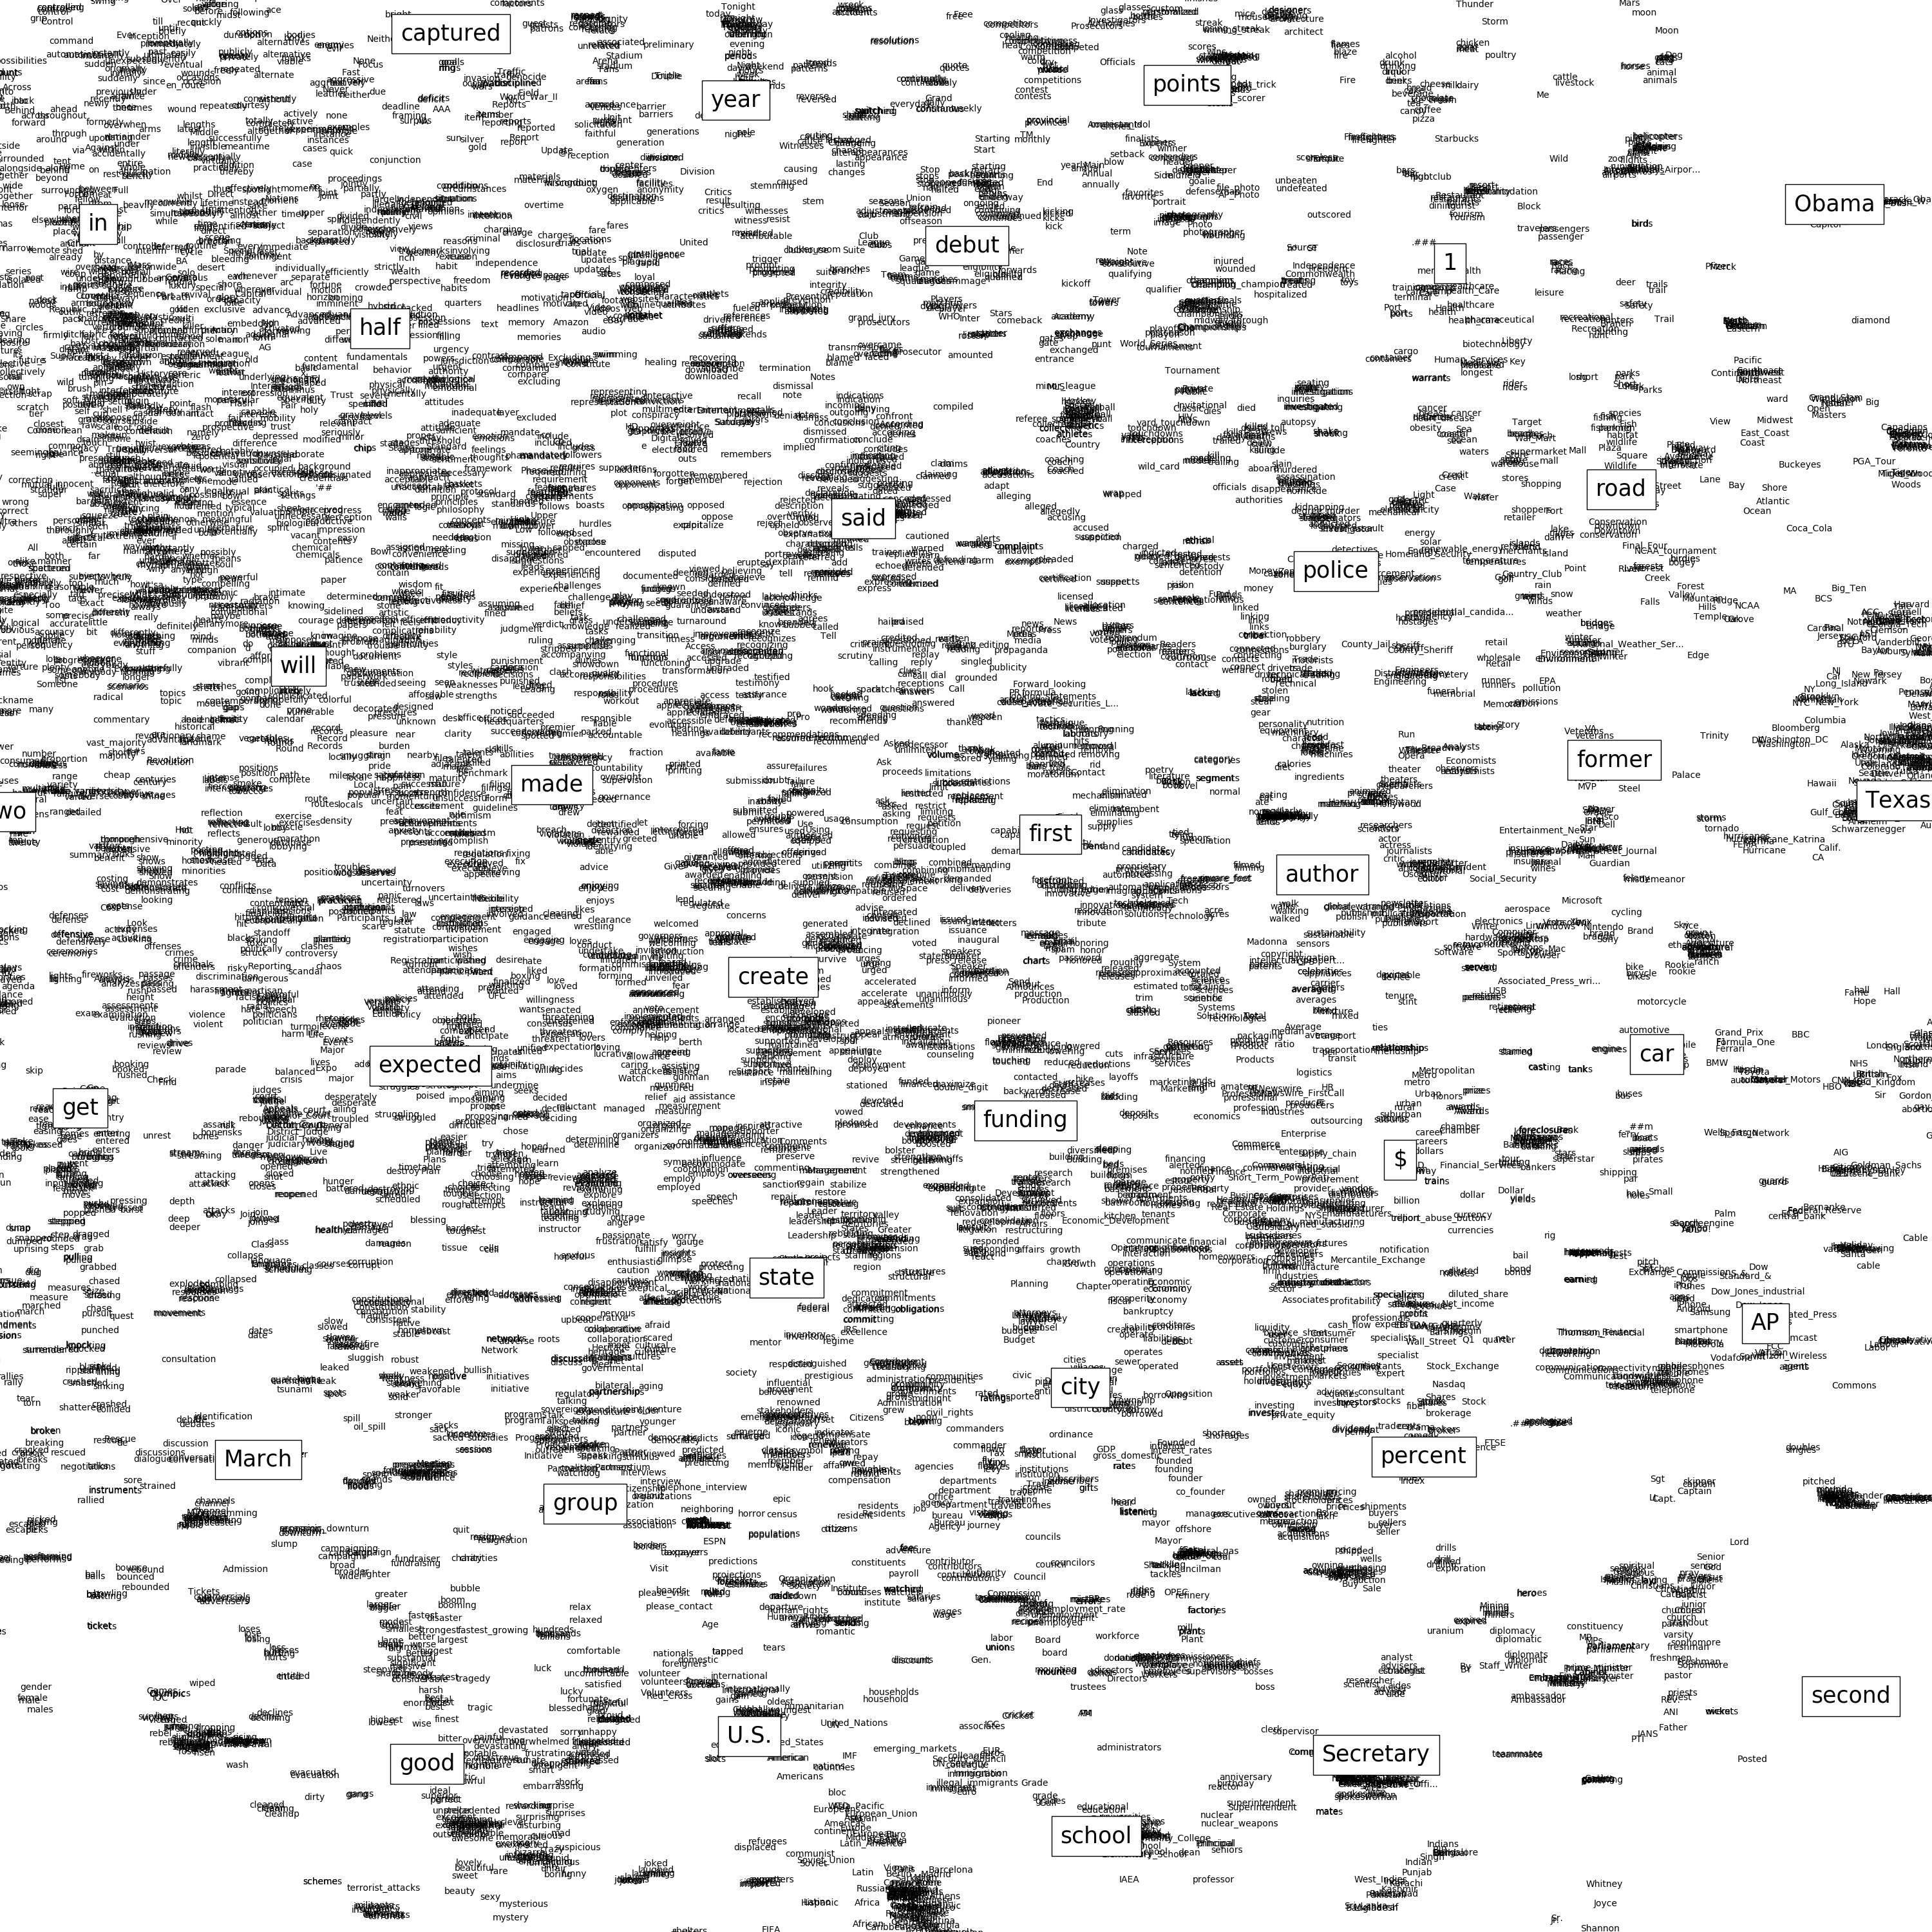
\includegraphics[height=0.9\textheight]{graph}

    \href[pdfnewwindow=true]{http://harvardnlp.github.io/seq2seq-talk/web/wordvecs.html}{[Words Vectors]}
   \end{center}
\end{frame}


\begin{frame}
  \begin{center}
    \begin{tabular}{cclll}
      \structure{RNNs/LSTMs} & & feature sequences & $\Rightarrow$ &dense features \\\\
    \end{tabular}
  \end{center}


  \begin{center}
    \includegraphics[width=11cm]{rnn}
  \end{center}  
\end{frame}



\begin{frame}
  \begin{center}
    \begin{tabular}{cclll}
      \structure{LM/Softmax} & & dense features & $\Rightarrow$ & discrete predictions \\
    \end{tabular}
    \air 

    \includegraphics[width=0.8\textwidth]{rnnlm5}
  \end{center}
  % \[ p(w_t | w_1, \ldots, w_{t-1}; \theta) = \text{softmax}(\mathbf{W}_{out} \mathbf{h}_{t-1} + \mathbf{b}_{out}) \] 

  % \[ p(w_{1:T} ) = \prod_{t} p(w_t | w_1, \ldots, w_{t-1}) \] 
  %   % \caption{Xu et al (2015)}  
\end{frame}

\begin{frame}
  \begin{center}
    \structure{Contextual Language Model / ``seq2seq''}
  \end{center}
    \air 
   
    \begin{center}
      \includegraphics[width=0.6\textwidth]{rnnlm6}
    \end{center}
  \begin{itemize}
  \item Key idea, contextual language model based on encoder $x$: 
  \end{itemize}
  % \[ p(w_{1:T} | x) = \prod_{t} p(w_t | w_1, \ldots, w_{t-1}, x) \] 
  
\end{frame}


\begin{frame}{Sequence-to-Sequence Models}
    \begin{center}
      \includegraphics[width=0.7\textwidth]{simple-attn}
    \end{center}
  % \begin{itemize}
  % \item Different encoders, attention mechanisms, input feeding, ...
  %   \air
  % \item Almost all models use LSTMs or other gated RNNs 
  %   \air
  % \item Large multi-layer networks  necessary for good performance.
  %   \begin{itemize}
  %   \item 4 layer, 1000 hidden dims is common for MT
  %   \end{itemize}
  % % \item Main idea, contextual language model based on encoder $\cvec$: 
  % \end{itemize}
  % \[ p(w_{1:T} | \cvec) = \prod_{t} p(w_t | w_1, \ldots, w_{t-1}, \cvec) \] 
\end{frame}


\begin{frame}{OpenNMT}
  \begin{itemize}
  \item Our open-source system  \href[pdfnewwindow=true]{http://opennmt.net}{http://opennmt.net}
    \air 
  \item Used by Systran in production system \Cite{systran}
  \item Most popular machine translation system on GitHub.
  \end{itemize}
  
  \begin{center}
    \includegraphics[width=0.8\textwidth]{systran}

    \href[pdfnewwindow=true]{http://demo-pnmt.systran.net}{[Demo]}
  \end{center}
\end{frame}

\section{Neural Summarization}


\begin{frame}{Neural Sentence Summarization \Cite{Rush2015}}
  % \centerline{\textbf{Seq2Seq Applications:} \alert{Neural Summarization} \Cite{Rush2015} }
  \begin{center}
    \textbf{Source} (First Sentence)
  \end{center}
  
  \begin{figure}
    \textit{\structure<2>{Russian Defense Minister Ivanov}
      called \structure<2>{Sunday} for the creation of
      a joint front \structure<2>{for combating} global terrorism. }
  \end{figure}

  \begin{center}
    \textbf{Target} (Title)
  \end{center}
  \mair

  \begin{figure}
    \centering
    \textit{\alert<2>{Russia} calls for joint
      front \alert<2>{against} terrorism.}
  \end{figure}
\end{frame}

\begin{frame}{Neural Summarization Model}
  \begin{itemize}
  \item System has since been replicated in many papers.
  \item Over 100 citations on dataset and model.
  \item Reimplemented in Tensorflow and OpenNMT

  \begin{center}
    \includegraphics[width=8cm]{onmtsum}
  \end{center}
  \item Used by Washington Post to suggest headlines \Cite{shuguangwang}
  \end{itemize}
\end{frame}


% \begin{frame}
%   \begin{itemize}
%   \item \Cite{mou2015backward} \Cite{cheng2016neural} \Cite{toutanovadataset} \Cite{wang2016experimental} \Cite{takaseneural}, among others
%   \item Used by Washington Post to suggest headlines \Cite{shuguangwang}
%   \end{itemize}
% \end{frame}



\begin{frame}{Extractive Neural Summarization \Cite{cheng2016neural}}
  \begin{itemize}
  \item Based on the DeepMind CNN/DailyMail data set. 
  \item Construct a large set of article and summaries.
  \item Utilize similar sequence-to-sequence models to learn extractive summaries.
  \end{itemize}
  \begin{center}
    \includegraphics[width=10cm]{chenglapa}
  \end{center}
\end{frame}


\begin{frame}{Pointer Networks \Cite{2015arXiv150603134V}}
  \begin{itemize}
  \item Many different recent papers have proposed hybrid copy/generation systems
  \item Several preliminary application to summarization \cite{zeng2016efficient}
  \item Useful for assuring named entity extraction.
  \end{itemize}
  \begin{center}
    \includegraphics[width=5cm]{ptrnet}
  \end{center}
\end{frame}

\begin{frame}{Multiple Domain Summarization \Cite{toutanovadataset}}
  \begin{itemize}
  \item Mechanical Turk dataset with summaries in 4 domains
  \item Showed that neural summarization is \textbf{not} very robust to domain changes.
      \includegraphics[width=10cm]{toutanova}
  \end{itemize}
\end{frame}


\begin{frame}{Semisupervised Summarization \Cite{miao2016language}}
  \begin{itemize}
  \item Summarization is very data hungry
  \item Hope is to use variational auto-encoders to regularize based on unlabeled data

  \end{itemize}
  \begin{center}
    \includegraphics[width=8cm]{textautoencoder}
  \end{center}
\end{frame}

\section{Proposed Research}

\begin{frame}{Samsung Interests}
  From conversation with Satish:
  \begin{itemize}
  \item Large document and dialog summarization.
  \item Interest in both Korean and English.
  \item Novel forms of memory for summarization.
  \end{itemize}
\end{frame}

\begin{frame}{Structured Attention \Cite{kim2017structured}}
  \begin{itemize}
  \item Novel method for attention at ICLR 2017.
  \item Allows probabilistic inference (CRF) within sequence-to-sequence.
  \item Applied to Japanese translation, question answering.
  \end{itemize}
  \begin{center}
    \includegraphics[width=7cm]{facts}
  \end{center}
  
\end{frame}

\begin{frame}{Proposed Project: Structured Attention for Summarization}
  \structure{Aim:} Summarize longer documents and maintaining information.
  \begin{itemize}
  \item Use structured attention with reinforcement learning to 
    do neural document summarization.
  \item Will select region of document to summarize, significantly 
    speed up summarization.
  \item Combined with pointer network, allows phrasal selection 
    in addition to abstractive embellishment.
  \end{itemize}
  \begin{center}
    \includegraphics[width=10cm]{structattn}
  \end{center}

\end{frame}



\begin{frame}{Project 2: Low-Resource Summarization}
  \begin{itemize}
  \item Aim: Learn neural summarization on fewer or unaligned summaries.
  \item Example: Languages with few summarized examples, 
    datasets with summarizations of the wrong size or form.
  \item Methodology: Utilize independent \structure{denoising autoencoders} in 
    original and summarized space. 
  \item Learn mapping from full representation to summarization.  
  \end{itemize}

  \begin{center}
    \includegraphics[width=7cm]{denoising}
  \end{center}
\end{frame}

\begin{frame}{Project 3: Structured Data Summarization}
  \begin{itemize}
    \item Aim: Learn long textual summarization of non-text input. 
    \item Example: Reports based on financial data, product descriptions based on 
      attribute specifications.
    \item Methodology: Use pointer network to select words and phrases, loss function 
      to ensure coherent generation.
  \end{itemize}

  \begin{center}
    \includegraphics[width=6cm]{booking}
  \end{center}
\end{frame}

% \begin{frame}
%   \centerline{\textbf{Seq2Seq Applications:} \alert{Im2Markup} (Deng and Rush, 2016) }
  
%   \air 

%   \begin{center}
%     \includegraphics[width=\textwidth]{math}
%   \end{center}
%   % \movie[width=\textwidth, height=4cm, poster, repeat]{}{Latex.mp4}
  


%   \begin{figure}
%     \centering
%   \end{figure}

%   \centerline{\href[pdfnewwindow=true]{https://harvardnlp.github.io/seq2seq-talk/web/math.html}{[Latex Example]}}
%   \centerline{\href[pdfnewwindow=true]{http://lstm.seas.harvard.edu/latex}{[Project]}}
% \end{frame}



% \begin{frame}
%   \centerline{\structure{This Talk}}
%   \air 
%   \air

%   \begin{itemize}
%   \item How can we \textbf{interpret} these learned hidden representations? 
%     \air 

    

%   \item  How should we \textbf{train} these style of models? 
%     \air 
%   \item  How can we \textbf{shrink} these models for practical applications? 
%   \end{itemize}
% \end{frame}


% \begin{frame}
%   \centerline{\structure{This Talk}}
%   \air 
%   \air

%   \begin{itemize}
%   \item How can we \textbf{interpret} these learned hidden representations? 

%     \begin{center}
%       \alert{LSTMVis}   
%       \href[pdfnewwindow=true]{https://lstm.seas.harvard.edu/}{lstm.seas.harvard.edu}

%       \Cite{Strobelt2016}

%       \includegraphics[width=2cm]{hen}
%     \end{center}


%     \air 

    

%   \item  \textcolor{gray}{How should we \textbf{train} these style of models? \Cite{Wiseman2016a}}
%     \air 
%   \item  \textcolor{gray}{How can we \textbf{shrink} these models for practical applications? \Cite{Kim2016a}}
%   \end{itemize}
% \end{frame}

% \section{Interpretation}

% % \begin{frame}
% %   \air 
% %   \includegraphics[width=\textwidth,trim={0 0 0 19.5cm},clip]{filters}
% %   \begin{center}
% %      \Cite{DBLP:conf/eccv/ZeilerF14}
% %   \end{center}
% % \end{frame}

% % \begin{frame}
% %   \begin{frame}
% %   \begin{center}
% %     \includegraphics[width=\textwidth]{lstm1}

% %     {\footnotesize (Karpathy et al, 2015)}
% %   \end{center}

% %     % \caption{Xu et al (2015)}  
% % \end{frame}

% \begin{frame}
%   \air 
%   \includegraphics[width=\textwidth,trim={0 0 0 19.5cm},clip]{filters}
%   \begin{center}
%      \Cite{DBLP:conf/eccv/ZeilerF14}
%   \end{center}
% \end{frame}


% \begin{frame}
%   % \begin{frame}
%   \centerline{Vector-Space RNN Representation}
%   \begin{center}
%     \includegraphics[height=5cm]{lstmrep}
%   \begin{center}
%     \includegraphics[width=11cm]{rnn}
%   \end{center}
%   \end{center}
% \end{frame}


% \begin{frame}
%   % \begin{frame}
%   \begin{center}
%     \includegraphics[width=\textwidth]{lstm1}

%      \Cite{karpathy2015visualizing}
%     % {\footnotesize (Karpathy et al, 2015)}
%   \end{center}
%     % \caption{Xu et al (2015)}  
% \end{frame}

% \begin{frame}
%   \centerline{\alert{Example 1}: Synthetic (Finite-State) Language}
%   \air

%   \begin{center}
%     \includegraphics[width=9cm]{parenlang}
%   \end{center}
%   \mair

%   \begin{itemize}
%   \item Numbers are randomly generated, must match nesting level.
%     \air

%   \item Train a predict-next-word language model (decoder-only).
%   \end{itemize}
%     \[ p(w_t | w_1, \ldots, w_{t-1}) \] 
  
% \air
%   \centerline{\href[pdfnewwindow=true]{http://lstm.seas.harvard.edu/client/pattern_finder.html?data_set=00parens&source=states::states2&pos=150}{[Parens Example]}}
% \end{frame}


% \begin{frame}
%   \centerline{\alert{Example 2}: Real Language}
%   \air

%   \begin{description}
%   \item[alphabet:] all english words
%   \item[corpus:] Project Gutenberg Children's books 
%   \end{description}
%   % \begin{center}
%   %   \includegraphics[width=9cm]{parenlang}
%   % \end{center}

%   \begin{itemize}
%   % \item 
%   %   \air

%   \item Train a predict-next-word language model (decoder-only).

  
%   \end{itemize}
%     \[ p(w_t | w_1, \ldots, w_{t-1}) \] 

% \air
%   \centerline{ \href[pdfnewwindow=true]{http://lstm.seas.harvard.edu/client/pattern_finder.html?data_set=05childbook&source=states::states1&pos=100}{[LM Example]}}
% \end{frame}


% \begin{frame}
%   \centerline{\alert{Example 3}: Seq2Seq Encoder}
%   \air

%   \begin{description}
%   \item[alphabet:] all english words
%   \item[corpus:]  Summarization
%   \end{description}
%   % \begin{center}
%   %   \includegraphics[width=9cm]{parenlang}
%   % \end{center}

%   \begin{itemize}
%   % \item 
%   %   \air

%   \item Train a full seq2seq model, examine \textit{encoder} LSTM.
  
%   \end{itemize}


% \air
%   \centerline{ \href[pdfnewwindow=true]{http://lstm.seas.harvard.edu/client/pattern_finder.html?data_set=20autoencoder&source=states::states2&pos=100}{[Summarization Example]}}
% \end{frame}
% \begin{frame}
%   \centerline{\structure{This Talk}}
%   \air 
%   \air

%   \begin{itemize}
%   \item \textcolor{gray}{How can we \textbf{interpret} these learned hidden representations? \Cite{Strobelt2016}}
%     \air 
%   \item  How should we \textbf{train} these style of models? 
%     \air 

%     \begin{center}
%       \alert{Sequence-to-Sequence Learning as Beam-Search
%         Optimization}
     
%       \Cite{Wiseman2016a}

%       \includegraphics[width=2cm]{sam}
%     \end{center}


%     \air 
%   \item \textcolor{gray}{ How can we \textbf{shrink} these models for practical applications \Cite{Kim2016a}? }
%   \end{itemize}
% \end{frame}

% \begin{frame}
%   % \centerline{Results}
%   \vspace{-0.2cm}
%   \begin{table}
%   \centering
%     \small
%   \begin{tabular}{lccc}
%     \toprule
%     & $K_e$ = 1 & $K_e$ = 5 & $K_e$ = 10 \\ 
%     \midrule
%      & \multicolumn{3}{c}{Word Ordering (BLEU) } \\ 
%     \midrule
%     seq2seq & 25.2 & 29.8 & 31.0 \\
%     BSO     & 28.0 & 33.2 & 34.3 \\
%     ConBSO & \textbf{28.6} & \textbf{34.3} & \textbf{34.5} \\
%     \midrule
% %   \end{tabular}
% %   \label{tab:wo}
% % \end{table}


% % \begin{table}
% %   \centering
% %   \hspace*{-0.3cm}\begin{tabular}{lccc}
% %     \toprule
%     & \multicolumn{3}{c}{Dependency Parsing (UAS/LAS)\footnote{Note \citet{Andor2016} have SOA, with 94.41/92.55.} } \\ 
%     % \midrule
%     seq2seq & \textbf{87.33/82.26} & 88.53/84.16 & 88.66/84.33\\
%     BSO & 86.91/82.11 & 91.00/\textbf{87.18} & 91.17/\textbf{87.41} \\
%     ConBSO & 85.11/79.32 & \textbf{91.25}/86.92 & \textbf{91.57}/87.26 \\
%     % \midrule
%     % Andor & 93.17/91.18 & - & - \\ 
%     % \bottomrule

%     \midrule
%     & \multicolumn{3}{c}{Machine Translation (BLEU) } \\ 
%     % &  $K_e$ = 1 & $K_e$ = 5 & $K_e$ = 10 \\ 
%     % \midrule
%     seq2seq & 22.53 & 24.03 & 23.87 \\
%     BSO, SB-$\Delta$, $K_t$=6 & \textbf{23.83} & \textbf{26.36} & \textbf{25.48} \\
%     % \midrule
%     XENT & 17.74 & 20.10 & 20.28 \\
%     DAD & 20.12 & 22.25 & 22.40 \\ 
%     MIXER & 20.73 & 21.81 & 21.83 \\    
%     \bottomrule
%   \end{tabular}
%   \label{tab:mtfinal}
% \end{table}

% \end{frame}


% \begin{frame}
%   \centerline{\structure{This Talk}}
%   \air 
%   \air

%   \begin{itemize}
%   \item \textcolor{gray}{How can we \textbf{interpret} these learned hidden representations? \Cite{Strobelt2016}}
%     \air 
%   \item  \textcolor{gray}{ How should we \textbf{train} these style of models? \Cite{Wiseman2016a}}
%     \air 
%   \item How can we \textbf{shrink} these models for practical applications?

%     \air 
%     \begin{center}
%       \alert{Sequence-Level Knowledge Distillation }

%       \Cite{Kim2016a} 

%       \includegraphics[width=2cm]{yoon}
%     \end{center}

%   \end{itemize}
% \end{frame}


% \begin{frame}
% \center
% \includegraphics[scale=0.5]{nmt-news} \\
% \end{frame}

% \begin{frame}
% \centerline{\structure{Neural Machine Translation}} \air \air
% Excellent results on many language pairs, but need large models \air
% \begin{itemize}
% \item Original seq2seq paper \Cite{Sutskever2014}: 4-layers/1000 units
% \item Deep Residual RNNs \Cite{Zhou2016} : 16-layers/512 units 
% \item Google's NMT system \Cite{Wu2016}: 8-layers/1024 units 
% \end{itemize}
% \air 
% \air 
% \pause
% Beam search + ensemble on top
% \\ 
% \air
% $\implies$ Deployment is challenging! 
% \end{frame}


% \begin{frame}
%   \centerline{\structure{Related Work: Compressing Deep Models}}
% \air
% \begin{itemize}
% \item \textbf{Pruning}: Prune weights based on importance criterion 
% \Cite{LeCun1990,Han2016,See2016}
% \item \textbf{Knowledge Distillation}: Train a \textit{student} model to learn 
% from a \textit{teacher} model \Cite{Bucila2006,Ba2014,Hinton2015,Kuncoro2016}. 
% (Sometimes called ``dark knowledge'')
% \end{itemize}
% % \air
% % \pause
% %  Other methods: 
% %  \begin{itemize}
% %  \item low-rank matrix factorization of weight matrices \Cite{Denton2014}
% %  \item weight binarization \Cite{Lin2016}
% %  \item weight sharing \Cite{Chen2015}
% %  \end{itemize}
% \end{frame}

% \begin{frame}
% \centerline{\structure{Knowledge Distillation \Cite{Bucila2006,Hinton2015}}}
% \air \air
% \begin{itemize}
% \item Train a \emph{larger teacher} model first to obtain teacher distribution $q(\cdot)$
% \item Train a \emph{smaller student} model $p(\cdot)$ to mimic the teacher 
% \end{itemize}
% % \\ \\
% % \air \air
% % \end{frame}

% % \begin{frame}
% \pause
% \air 
% \alert{Word-Level Knowledge Distillation}
% \air

% Teacher distribution: $q(w_t \given y_{1:t-1})$ 
% \begin{align*}
% \mathcal{L}_{\text{NLL}} &=- \sum_t \sum_{k \in \mathcal{V}} {\color{red}{\mathbbm{1}\{y_t = k\}}} \log p(w_t = k \given  y_{1:t-1}; \theta) \\
% \mathcal{L}_{\text{WORD-KD}} &=- \sum_t \sum_{k \in \mathcal{V}} {\color{blue}{q(w_t = k \given y_{1:t-1})}} \log p(w_t = k \given  y_{1:t-1}; \theta)
% \end{align*}
% \end{frame}

% \begin{frame}
% \centerline{\structure{No Knowledge Distillation}}
% \air 
% \center
% \includegraphics[width=6cm]{word-kd-0}
% \end{frame}

% \begin{frame}
% \centerline{\structure{Word-Level Knowledge Distillation}}
% \air 
% \begin{figure}
% \center
% \includegraphics[width=6cm]{word-kd-1}
% \end{figure}
% \end{frame}

% \begin{frame}
% \centerline{\structure{Word-Level Knowledge Distillation}}
% \air
% \begin{figure} 
% \center
% \includegraphics[width=6cm]{word-kd-2}
% \end{figure}
% \end{frame}

% % \begin{frame}
% % \centerline{\structure{Word-Level Knowledge Distillation}}
% % \air 
% % \center
% % \includegraphics[width=5.5cm]{word-kd-3}
% % $$\mathcal{L} = \alpha{\color{blue}{\mathcal{L}_{\text{WORD-KD}}}} + (1-\alpha){\color{red}{\mathcal{L}_{\text{NLL}}}}$$
% % \end{frame}

% % \begin{frame}
% % \centerline{\structure{Baseline Model (No Knowledge Distillation)}}
% % \air 

% % \begin{columns}
% % \begin{column}{6.5cm}
% % Minimize NLL
% % $$\mathcal{L}_{\text{NLL}} = -\sum_t \log p(y_t=\hat{y}_t \given \yvec_{1:t-1}, \xvec ; \theta)$$
% % $y_t$ = $t$-th target token \\
% % $\yvec_{1:t-1}$ = target sentence up to $t-1$ \\
% % $\xvec$  = source sentence \\
% % \air \air
% % (conditioning on source $\xvec$ dropped from now on)
% % \end{column}
% % \begin{column}{5.5cm}
% % \includegraphics[width=5.5cm]{word-kd-0}
% % \end{column}
% % \end{columns}
% % \end{frame}

% % \begin{frame}
% % \centerline{\structure{Word-Level Knowledge Distillation}}
% % \air 
% % \air

% % \begin{columns}
% % \begin{column}{6.5cm}
% % Teacher network: $q(y_t \given \yvec_{1:t-1} ; \theta_T$)  \\
% % \air
% % \air
% % Student network: $p(y_t \given \yvec_{1:t-1} ; \theta$)
% % \end{column}
% % \begin{column}{5.5cm}
% % \includegraphics[width=5.5cm]{word-kd-1}
% % \end{column}
% % \end{columns}
% % \end{frame}


% % \begin{frame}

% % \centerline{\structure{Word-Level Knowledge Distillation}}
% % \air 
% % \begin{columns}
% % \begin{column}{6.5cm}

% % Teacher network: $q(y_t | \yvec_{1:t-1}  ; \theta_T$)  
% % \air 

% % Minimize cross-entropy with teacher 
% % \begin{align*}
% % \mathcal{L}_{\text{WORD-KD}} = &  \\ -\sum_t \sum_{k \in \mathcal{V}} &q(y_t=k \given \yvec_{1: t-1} ; \theta_T)\times \\
% % & \log p(y_t =k \given \yvec_{1: t-1} ; \theta)
% % \end{align*}
% % Sometimes $q$ and $p$ are annealed (i.e. $\tilde{q} \propto q^{\frac{1}{\tau}}$) to make it less peaky
% % \end{column}

% % \begin{column}{5.5cm}
% % \includegraphics[width=5.5cm]{word-kd-2}
% % \end{column}
% % \end{columns}
% % \end{frame}

% % \begin{frame}
% % \centerline{\structure{Word-Level Knowledge Distillation}}
% % \air
% % \begin{columns}
% % \begin{column}{6.5cm}
% % Add a term for NLL 
% % $$\mathcal{L} = \alpha\mathcal{L}_{\text{WORD-KD}} + (1-\alpha)\mathcal{L}_{\text{NLL}}$$
% % \air
% % (we use $\alpha = 0.5$)
% % \end{column}

% % \begin{column}{5.5cm}
% % \includegraphics[width=5.5cm]{word-kd-3}
% % \end{column}
% % \end{columns}
% % \end{frame}

% \begin{frame}
% \centerline{\structure{Word-Level Knowledge Distillation Results}}
% \air
% \air
% \center English $\rightarrow$ German (WMT 2014)
% \begin{table}
% \centering
% \small
% \begin{tabular}{lc}
% \toprule
% Model &  BLEU   \\
% \midrule
% $4 \times 1000$  Teacher    &  $19.5$ \\
% \midrule
% $2 \times 500$ Baseline (No-KD)  $\,$   &  $17.6$   \\
% $2 \times 500$ Student (Word-KD)  & $17.7$   \\
% \midrule 
% $2 \times 300$  Baseline (No-KD)  $\,$   &  $16.9$  \\
% $2 \times 300$  Student (Word-KD)  &  $17.6$  \\
% \bottomrule
% \end{tabular}
% \end{table}
% \end{frame}

% % \begin{frame}
% % \centerline{\structure{This Work}}
% % \air 
% % \air
% % Generalize single-class knowledge distillation to the sequence-level.
% % \begin{itemize}
% % \item \textbf{Sequence-Level Knowledge Distillation (Seq-KD)}: Train towards the teacher's sequence-level
% % distribution.
% % \item \textbf{Sequence-Level Interpolation (Seq-Inter)}: Train on a mixture of the teacher's distribution and the data.
% % \end{itemize}
% % \end{frame}

% \begin{frame}
% \centerline{\structure{This Work:  Sequence-Level Knowledge Distillation}}
% \air 
% \begin{align*}
% \mathcal{L}_{\text{NLL}} &=- \sum_t \sum_{k \in \mathcal{V}} {\color{red}{\mathbbm{1}\{y_t = k\}}} \log p(w_t = k \given  y_{1:t-1}) \\
% \mathcal{L}_{\text{WORD-KD}} &=- \sum_t \sum_{k \in \mathcal{V}} {\color{blue}{q(w_t = k \given y_{1:t-1})}} \log p(w_t = k \given  y_{1:t-1})
% \end{align*}
% \pause
% Instead minimize cross-entropy, between $q$ and $p$ implied \emph{sequence}-distributions 
% \begin{align*}
% \mathcal{L}_\text{SEQ-KD} &=  -\sum_{w_{1:T} \in \mathcal{V}^T}{\color{blue}{q(w_{1:T} \given x)}}  \log p(w_{1:T} \given x  )
% \end{align*}
% \air
% Sum over an exponentially-sized set $\mathcal{V}^T$. 
% \end{frame}

% \begin{frame}
% \centerline{\structure{Sequence-Level Knowledge Distillation}}
% \air 
% \air
% Approximate $q(w \given x )$ with mode
% $$q(w_{1:T} \given x) \approx \mathbbm{1}\{\argmax_{w_{1:T}} q(w_{1:T} \given x )\}$$
% \air
% \pause
% Approximate mode with  beam search 
% $$ \hat{y} \approx  \argmax_{w_{1:T}} q(w_{1:T} \given x) $$
% \pause
% % Empirically, point estimate captures significant mass \\
% % (Other approximations possible)

% Simple model: train the student model on $\hat{y}$ with NLL
% \end{frame}


% \begin{frame}
% \centerline{\structure{Sequence-Level Knowledge Distillation}}
% \air 
% \air
% \begin{figure}
% \center
% \includegraphics[width=7.5cm]{seq-kd-1}
% \end{figure}
% \end{frame}

% \begin{frame}
% \centerline{\structure{Sequence-Level Knowledge Distillation}}
% \air
% \air  
% \begin{figure}
% \center
% \includegraphics[width=7.5cm]{seq-kd-2}
% \end{figure}
% \end{frame}

% \begin{frame}
% \centerline{\structure{Sequence-Level Interpolation}}
% \air \air \air
% Word-level knowledge distillation
% \[ \mathcal{L} = \alpha{\color{blue}{\mathcal{L}_{\text{WORD-KD}}}} + (1-\alpha)\color{red}{\mathcal{L}_{\text{NLL}}}\]
% Training the student towards the mixture of teacher/data distributions. \\
% \air \air
% How can we incorporate ground truth data at the sequence-level?
% \end{frame}


% \begin{frame}
% \centerline{\structure{Sequence-Level Interpolation}}
% \air \air
% \begin{figure}
% \center
% \includegraphics[width=7.5cm]{seq-inter-0}
% \end{figure}
% \end{frame}

% \begin{frame}
% \centerline{\structure{Sequence-Level Interpolation}}
% \air \air
% \begin{figure}
% \center
% \includegraphics[width=7.5cm]{seq-inter-1}
% \end{figure}
% \end{frame}


% \begin{frame}
% \centerline{\structure{Experiments on English $\rightarrow$ German (WMT 2014)}}
% \begin{itemize}
% \item Word-KD: Word-level Knowledge Distillation
% \item Seq-KD: Sequence-level Knowledge Distillation with beam size $K=5$
% \item Seq-Inter: Sequence-level Interpolation with beam size $K=35$. Fine-tune
% from pretrained Seq-KD (or baseline) model with smaller learning rate.
% \end{itemize}
% % Can mix configurations (e.g. train on Seq-KD data with word-level cross
% % entropy against teacher)
% \end{frame}

% \begin{frame}
% \centerline{\structure{Results: English $\rightarrow$ German (WMT 2014)}}
% \air
% \air
% \begin{table}
% \centering
% \small
% \begin{tabular}{lccccrr}
% \toprule
% Model &    BLEU$_{K=1}$   & $\Delta_{K=1}$ & BLEU$_{K=5}$ & $\Delta_{K=5}$ &  PPL & $p(\hat{\yvec})$ \\
% \midrule
% $4 \times 1000$ \\
% Teacher    & $17.7$ &  $-$ & $19.5$&   $-$ &    $6.7$ &  $1.3\%$ \\
% \only<5->{\hspace{1mm} Seq-Inter    & $19.6$ & $+1.9$&  $19.8$& $+0.3$&    $10.4$ & $8.2\%$}   \\
% \midrule
% $2 \times 500$ \\ 
% Student  $\,$   & $14.7$ & $-$ & $17.6$&  $-$ &   $8.2$ & $0.9\%$  \\
% \only<2->{\hspace{1mm} Word-KD  & $15.4$ & $+0.7$& $17.7$& $+0.1$&   $8.0$ & $1.0\%$}  \\
% \only<3->{\hspace{1mm} Seq-KD   & $18.9$ & $+4.2$& $19.0$& $+1.4$&   $22.7$ & $16.9\%$} \\
% \only<4->{\hspace{1mm} Seq-Inter  & $18.9$ & $+4.2$&$19.3$ & $+1.7$ &   $15.8$ & $7.6\%$}  \\
% \bottomrule
% \end{tabular}
% \end{table}
% \only<6>{\small Many more experiments (different language pairs, combining configurations, different sizes etc.) in paper}
% \end{frame}

% \begin{frame}
% \centerline{\structure{An Application}}
% \begin{center}

% \includegraphics[width=5cm]{phonemt}
%   \end{center}

%   \href[pdfnewwindow=true]{https://harvardnlp.github.io/seq2seq-talk/transfast.gif}{[App]}
% \end{frame}


% \begin{frame}
% \centerline{\structure{Decoding Speed}}
% \center
% \vspace{-5mm}
% \includegraphics[scale=0.44]{dec-speed.pdf}
% \end{frame}


% \begin{frame}
% \centerline{\structure{Combining Knowledge Distillation and Pruning}}
% \air
% \air
% Number of parameters still large for student models (mostly due to word embedding tables)
% \begin{itemize}
% \item $4 \times 1000$: $221$ million
% \item $2 \times 500$: $84$ million
% \item $2 \times 300$: $49$ million
% \end{itemize}
% \\ \air
% \pause
% Prune student model: Same methodology as \cite{See2016}
% \begin{itemize}
% \item Prune $x\%$ of weights based on absolute value
% \item Fine-tune pruned model (crucial!)
% \end{itemize}
% \end{frame}

% \begin{frame}
% \centerline{\structure{Combining Knowledge Distillation and Pruning}}
% \air
% \air
% \includegraphics[scale=0.4]{size}
% \end{frame}

% \begin{frame}
% \centerline{\structure{Conclusion: Other work}}
%   \begin{itemize}
%   \item How can we \textbf{interpret} these learned hidden representations? 
%     \air 

% \begin{itemize}
%     \item Lei et al. (2016) other methods for interpreting decisions (as opposed to states).
% \end{itemize}


%   \item  How should we \textbf{train} these style of models? 

% \begin{itemize}
%     \item Lee et al. (2016) CCG parsing (backprop through search is a thing now/again)

% \end{itemize}

%   \item  How can we \textbf{shrink} these models for practical applications? 

%     \begin{itemize}
%     \item  Live deployment: (greedy) student outperforms (beam search) teacher. \Cite{systran}  
%     \item Can compress an ensemble into a single model \Cite{Kuncoro2016}
%     \end{itemize}
%   \end{itemize}
% \end{frame}

% \begin{frame}
%   \begin{center}
%     \textbf{Coming Work}    
%   \end{center}

%   \begin{itemize}
%   \item Structured Attention Networks (Kim et al 2016)
%   \end{itemize}

%   \begin{figure}
%   \centering
%   \begin{subfigure}{0.32\textwidth}
%     \centering
%   \begin{tikzpicture}
%     \tikzstyle{latent} = [circle,fill=white,draw=black,inner sep=1pt,
%     minimum size=20pt, font=\fontsize{10}{10}\selectfont]
%     \tikzstyle{obs} = [latent,fill=gray!25]

%     \node[obs](q){$q$};
%     \node[below of=q, latent](za){$z_1$};
%     \node[xshift= -1.5cm,below of=za, obs](xa){$x_1$};
%     \node[right of=xa, obs](xb){$x_2$};
%     \node[right of=xb, obs](xc){$x_3$};
%     \node[right of=xc, obs](xd){$x_4$};

%     \draw[dashed] (xa) to (za);
%     \draw[dashed] (xb) to (za);
%     \draw[dashed] (xc) to (za);
%     \draw[dashed] (xd) to (za);
%   \end{tikzpicture}
%   \caption{}
%   \end{subfigure}
%   \begin{subfigure}{0.32\textwidth}
%     \centering
%   \begin{tikzpicture}
%     \tikzstyle{latent} = [circle,fill=white,draw=black,inner sep=1pt,
%     minimum size=20pt, font=\fontsize{10}{10}\selectfont]
%     \tikzstyle{obs} = [latent,fill=gray!25]

%     \node[obs](q){$q$};
%     \node[xshift= -1.5cm, below of=q, latent](za){$z_1$};
%     \node[right of=za, latent](zb){$z_2$};
%     \node[right of=zb, latent](zc){$z_3$};
%     \node[right of=zc, latent](zd){$z_4$};
%     \node[below of=za, obs](xa){$x_1$};
%     \node[below of=zb, obs](xb){$x_2$};
%     \node[below of=zc, obs](xc){$x_3$};
%     \node[below of=zd, obs](xd){$x_4$};

%     % \draw (za) to (zb);
%     % \draw (zb) to (zc);
%     % \draw (zc) to (zd);

%     \draw[dashed] (xa) to (za);
%     \draw[dashed] (xb) to (zb);
%     \draw[dashed] (xc) to (zc);
%     \draw[dashed] (xd) to (zd);
%   \end{tikzpicture}
%   \caption{}
%   \end{subfigure}
%   \begin{subfigure}{0.3\textwidth}
%     \centering
%   \begin{tikzpicture}
%     \tikzstyle{latent} = [circle,fill=white,draw=black,inner sep=1pt,
%     minimum size=20pt, font=\fontsize{10}{10}\selectfont]
%     \tikzstyle{obs} = [latent,fill=gray!25]

%     \node[obs](q){$q$};
%     \node[xshift= -1.5cm, below of=q, latent](za){$z_1$};
%     \node[right of=za, latent](zb){$z_2$};
%     \node[right of=zb, latent](zc){$z_3$};
%     \node[right of=zc, latent](zd){$z_4$};
%     \node[below of=za, obs](xa){$x_1$};
%     \node[below of=zb, obs](xb){$x_2$};
%     \node[below of=zc, obs](xc){$x_3$};
%     \node[below of=zd, obs](xd){$x_4$};

%     \draw[line width=1] (za) to (zb);
%     \draw[line width=1] (zb) to (zc);
%     \draw[line width=1] (zc) to (zd);

%     \draw[dashed] (xa) to (za);
%     \draw[dashed] (xb) to (zb);
%     \draw[dashed] (xc) to (zc);
%     \draw[dashed] (xd) to (zd);
%   \end{tikzpicture}
%   \caption{}
%   \end{subfigure}

% % \includegraphics[scale=0.3]{linear-crf}
%  %  \caption{\small \label{fig:seq} Three versions of a latent variable attention
%  %    model:
%  % (a) A standard soft-selection attention network, (b) A
%  %    Bernoulli (sigmoid) attention network, (c) A linear-chain
%  %    structured attention model for segmentation. The input and query are denoted with $x$ and $q$ respectively. }
% \end{figure}

% \end{frame}


% % \begin{frame}
% % \frametitle{Conclusion}
% % Introduced a variant of Seq2Seq and training procedure that:
% % \begin{itemize}
% % \air
% % \item Attempts to mitigate Label Bias and Exposure Bias
% % \air
% % \item Allows tuning to test-time metrics
% % \air
% % \item Allows training with hard constraints
% % \air
% % \item Doesn't require RL
% % \end{itemize}

% % \air
% % \air
% % \textbf{N.B.} Backprop through search is a thing now/again:
% % \begin{itemize}
% % \item One piece of the CCG parsing approach of Lee et al. (2016), an EMNLP 2016 Best Paper!
% % \end{itemize}
% % \end{frame}

% \begin{frame}
% \begin{center}
% Thanks!
% \end{center}
% \end{frame}


% \begin{frame}
%   \begin{center} 
%     \structure{Thank You}
%   \end{center}
%   \air 
%   \begin{center}
%     \includegraphics[width=3cm]{harvardnlp}
%   \end{center}
%   % \structure{Focus:} Deep learning of the representation of language structure

%   \begin{center}
%     \includegraphics[width=6cm]{harvardnlpgroup}
%   \end{center}
  
% \end{frame}



\begin{frame}[t,allowframebreaks]
  \frametitle{References}
  \begin{small}
    \bibliography{full,career2,seq2seqapps,ourwork,master,masterseqk,beamtrain}
  \end{small}
 \end{frame}

\bibliographystyle{apalike}

\end{document}
